% Copyright (c) 2020-2021 Robert Ryszard Paciorek <rrp@opcode.eu.org>
% 
% MIT License
% 
% Permission is hereby granted, free of charge, to any person obtaining a copy
% of this software and associated documentation files (the "Software"), to deal
% in the Software without restriction, including without limitation the rights
% to use, copy, modify, merge, publish, distribute, sublicense, and/or sell
% copies of the Software, and to permit persons to whom the Software is
% furnished to do so, subject to the following conditions:
% 
% The above copyright notice and this permission notice shall be included in all
% copies or substantial portions of the Software.
% 
% THE SOFTWARE IS PROVIDED "AS IS", WITHOUT WARRANTY OF ANY KIND, EXPRESS OR
% IMPLIED, INCLUDING BUT NOT LIMITED TO THE WARRANTIES OF MERCHANTABILITY,
% FITNESS FOR A PARTICULAR PURPOSE AND NONINFRINGEMENT. IN NO EVENT SHALL THE
% AUTHORS OR COPYRIGHT HOLDERS BE LIABLE FOR ANY CLAIM, DAMAGES OR OTHER
% LIABILITY, WHETHER IN AN ACTION OF CONTRACT, TORT OR OTHERWISE, ARISING FROM,
% OUT OF OR IN CONNECTION WITH THE SOFTWARE OR THE USE OR OTHER DEALINGS IN THE
% SOFTWARE.

\documentclass{pdfBooklets}

\title{Linux i sieci: Podstawowe polecenia Unix'a}
\author{%
	Projekt ,,Matematyka dla Ciekawych Świata'',\\
	Robert Ryszard Paciorek\\\normalsize\ttfamily <rrp@opcode.eu.org>
}
\date  {2024-10-03}

\makeatletter\hypersetup{
	pdftitle = {\@title}, pdfauthor = {\@author}
}\makeatother

\begin{document}

\maketitle

% Copyright (c) 2017-2020 Matematyka dla Ciekawych Świata (http://ciekawi.icm.edu.pl/)
% Copyright (c) 2017-2020 Robert Ryszard Paciorek <rrp@opcode.eu.org>
% 
% MIT License
% 
% Permission is hereby granted, free of charge, to any person obtaining a copy
% of this software and associated documentation files (the "Software"), to deal
% in the Software without restriction, including without limitation the rights
% to use, copy, modify, merge, publish, distribute, sublicense, and/or sell
% copies of the Software, and to permit persons to whom the Software is
% furnished to do so, subject to the following conditions:
% 
% The above copyright notice and this permission notice shall be included in all
% copies or substantial portions of the Software.
% 
% THE SOFTWARE IS PROVIDED "AS IS", WITHOUT WARRANTY OF ANY KIND, EXPRESS OR
% IMPLIED, INCLUDING BUT NOT LIMITED TO THE WARRANTIES OF MERCHANTABILITY,
% FITNESS FOR A PARTICULAR PURPOSE AND NONINFRINGEMENT. IN NO EVENT SHALL THE
% AUTHORS OR COPYRIGHT HOLDERS BE LIABLE FOR ANY CLAIM, DAMAGES OR OTHER
% LIABILITY, WHETHER IN AN ACTION OF CONTRACT, TORT OR OTHERWISE, ARISING FROM,
% OUT OF OR IN CONNECTION WITH THE SOFTWARE OR THE USE OR OTHER DEALINGS IN THE
% SOFTWARE.

% BEGIN: unix intro
\section{Praca w terminalu}

Komputer potrafi jedynie wykonywać jakiś wcześniej zaprogramowany ciąg instrukcji.
Każde wydane przez użytkownika polecenie wiąże się z uruchomieniem takiego ciągu instrukcji (programu komputerowego lub jakieś funkcji w ramach niego).

Podstawowym sposobem wydawania poleceń w systemach typu Unix jest wpisywanie ich w terminalu.
Terminal może pracować w trybie tekstowym lub może być uruchomiony (jako tzw. emulator terminala) w trybie graficznym.

\subsection{Powłoka}

Wprowadzane polecenia interpretowane są przez działający w terminalu program nazywany powłoką (interpreterem poleceń).
W terminalu mogą być uruchamiane kolejne (takie same lub różne) interpretery poleceń.
Różne interpretery korzystają z różnych składni oraz często różnią się znakiem zachęty (czyli wypisanym tekstem poprzedzającym wprowadzane polecenia).

\subsubsection{bash}
Bash jest chyba najpopularniejszą powłoką (interpreterem poleceń) systemową w środowiskach linuksowych.
Jest zgodny ze składnią z sh, zapewnia m.in. obsługę zmiennych (zasadniczo napisowych) oraz omówionych w dalszej części skryptu znaków uogólniających.

\begin{ProTip}[breakable]{Edycja i historia linii poleceń}
Bash, podobnie jak wiele innych interpreterów poleceń (np. Python) umożliwia edycję linii poleceń oraz korzystanie z jej historii.\footnote{
	Bash korzysta w tym celu z popularnej biblioteki \textit{GNU Readline} (więcej na jej temat: \url{https://en.wikipedia.org/wiki/GNU\_Readline}).
	Biblioteka ta może zostać użyta w kodzie programu do obsługi wejścia, ale może zostać dodana do także zewnętrznie przy pomocy np. \Verb$rlwrap$.
}
Poruszanie się po historii linii poleceń możliwe jest strzałkami góra/dół, wyszukiwanie w historii przy pomocy Ctrl+R.
Dostępne jest też polecenie wbudowane \texttt{history} umożliwiające wypisanie całej zapamiętanej historii oraz zarządzanie nią.

Bash pozwala także na dopełnianie nazw poleceń i ścieżek (a po odpowiedniej konfiguracji – pakiet \textit{bash-completion} – także innych argumentów poleceń) przy pomocy tabulatora.
\end{ProTip}

\subsubsection{screen i tmux}
\texttt{screen} i \texttt{tmux} są tzw. multiplexerami terminala - pozwala na uzyskanie wielu okien konsoli (także np. wyświetlanych jedno obok drugiego) na pojedynczym terminalu.
Ponadto pozwalają na odłączanie i podłączanie sesji, co pozwala na łatwe pozostawienie działającego programu po wylogowaniu i powrót do niego później.

\subsection{Komendy}

Unixowe komendy (czyli polecenia rozumiane przez bash lub inny interpreter zgodny z sh) składają się z nazwy polecenia oraz opcji i argumentów.
Nazwą polecenia może być nazwa funkcji wbudowanej, nazwa programu (znajdującego się w ścieżce wyszukiwania programów) lub pełna ścieżka do programu.
Po nazwie polecenia mogą występować opcje i/lub argumenty. Są one oddzielane od nazwy polecenia i od siebie przy pomocy spacji\footnote{
	zasadniczo dowolnego ciągu białych znaków: spacji, tabulatorów, ,,escapowanych'' nowych linii.
}.
Nie ma silnego rozróżnienia opcji od argumentów, typowo stosowaną konwencją jest rozpoczynanie opcji od pojedynczego myślnika (opcje krótkie - jednoliterowe) lub dwóch myślników (opcje długie).
	W przypadku stosowania tej konwencji po pojedynczym myślniku może występować kilka bezargumentowych opcji jednoliterowych.
	Typowo argumenty opcji oddzielane są od nich spacją (w przypadku opcji krótkich) lub znakiem równości (w przypadku opcji długich).
Jeżeli któryś z składników komendy (np. argument) zawiera spacje należy je zabezpieczyć przy pomocy odwrotnego ukośnika lub ujęcia zawierającego je napisu w apostrofy lub cudzysłowia.

\subsection{Uzyskiwanie pomocy}

Informację na temat działania danej komendy oraz jej opcji można uzyskać w wbudowanym systemie pomocy przy pomocy poleceń \Verb{man} lub \Verb{info} / \Verb{pinfo}.
Większość poleceń obsługuje także opcje \Verb{--help} lub \Verb{-h}, które wyświetlają informację na temat ich użycia.

\pagebreak[2]\begin{ProTip}{Notacja}
Zarówno w tekstach pomocy jak i w tym dokumencie stosowana jest konwencja polegająca na oznaczaniu opcjonalnych argumentów poprzez umieszczanie ich w nawiasach kwadartowych (jeżeli podajemy ten argument do komendy nie obejmujemy go już tymi nawiasami) oraz rozdzielaniu alternatywnych opcji przy pomocy~\Verb{|}. Np. \Verb{a [b] c|d} oznacza iż polecenie \Verb{a} wymaga argumentu postaci \Verb{c} albo \Verb{d}, który może być poprzedzony argumentem \Verb{b}.
\end{ProTip}

\subsection{more i less}

Jeżeli wynik jakiejś komendy nie mieści się na ekranie do jego obejrzenia możemy użyć poleceń \Verb{more} lub \Verb{less}. Są to programy umożliwiające przeglądanie tekstu ekran po ekranie.
\Verb{less} posiada większe możliwości od more (w szczególności posiada możliwość przeglądanie dokumentu w tył)\footnote{
wybrane przydatne opcje:
	\Verb{-X} nie czyści ekranu przy wychodzeniu z less'a (całość historii wyświetlania pliku pozostaje w historii terminala)
	\Verb{-F} automatycznie kończy gdy wyświetlany tekst mieści się na jednym ekranie
}. Programy te kończą się po wciśnięciu klawisza \Verb{q}. \Verb{less} umożliwia także wyszukiwanie -- klawisz \Verb{/} pozwala na wprowadzenie szukanej frazy, a \Verb{n} na wyszukanie kolejnego wystąpienia.
Programy te umożliwiają też wyświetlanie wskazanych jako argumenty plików.

\subsection{Przekierowania}

Typowo program posiada trzy strumienie danych: jednen wejściowy (stdin) i dwa wyjściowe (stdout i stderr). Standardowe wyjście możemy przekierować na standardowe wejście innego programu przy pomocy~\Verb{|}, np:
\begin{Verbatim}
ls --help | less
\end{Verbatim}
Konstrukcja ta przekieruje wynik komendy \Verb{ls} uruchomionej z opcją \Verb{--help} do komendy \Verb{less}.

Możemy także przekierować standardowe wyjście do pliku (przy pomocy~\Verb{>} lub~\Verb{>>}, gdy chcemy dopisywać do pliku) lub pobrać standardowe wejście z pliku (przy pomocy \Verb{<}).
\Verb{2>} pozwala na przekierowanie standardowego wyjścia błędu do pliku, a \Verb{>&} i \Verb{|&} pozwala na przekierowanie obu strumieni odpowiednio do pliku lub standardowego wejścia innego polecenia.
% END: unix intro

\subsection{Kod powrotu polecenia oraz łączenie poleceń}

Każde uruchamiane polecenie po zakończeniu działania zwraca liczbowy kod powrotu (w przypadku programów w C jest to wartość zwracana z funkcji \Verb$main$).
Zero oznacza że polecenie zakończyło się sukcesem (np. znaleziono szukane pliki), wartość nie zerowa że zakończyło się porażką (np. nie ma pasujących plików) lub błędem (np. składnia wprowadzonego polecenia była niepoprawna).

Polecenia mogą być łączone na różne sposoby – z wykorzystaniem tej informacji lub nie:
\begin{itemize}
	\item \Verb$a && b$ – polecenie b wykona się gdy a zakończyło się sukcesem (zwróciło kod 0)
	\item \Verb$a || b$ – polecenie b wykona się gdy a zakończyło się porażką lub błędem (zwróciło kod różny od~0)
	\item \Verb$a ; b$ – polecenie b po zakończeniu polecenia a (bez względu na jego kod powrotu)
	\item \Verb$a & b$ – polecenie b będzie wykonywane równocześnie z a (dokładniej polecenie a zostanie uruchomione w tle, a na terminal zajmie polecenie b)
\end{itemize}

Spacje w powyższych konstrukcjach są opcjonalne.
Średnik i pojedynczy \Verb$&$ mogą być dodane do polecenia także gdy nie ma kolejnego w ciągu:
\begin{itemize}
	\item \Verb$a&$ uruchomi polecenie a w tle i odda linię poleceń,
	\item \Verb$a;$ uruchomi polecenie a (dokładnie tak samo jakby nie było tego średnika).
\end{itemize}

% BEGIN: katalog roboczy
\subsection{Katalog roboczy}

System plików ma strukturę hierarchiczną (drzewiastą) i rozpoczyna się w korzeniu oznaczanym ukośnikiem: \texttt{/}.
Możliwe jest wyrażanie wszystkich ścieżek od korzenia, jednak nie jest to zbytnio wygodne.
Interpreter poleceń taki jak \textit{bash} potrafi znajdować się gdzieś w tej strukturze plików i miejsce to nazywane jest bieżącym katalogiem roboczym (\textit{Present Working Directory}).
Względem niego będą wyrażane ścieżki nie zaczynające się od korzenia, może być też oznaczony jawnie przy pomocy pojedynczej kropki.

\begin{itemize}
	\item \Verb{cd [ścieżka]}
		zmiana bieżącego katalogu,\\
			warto zauważyć, iż katalogi w ścieżce oddzielamy ukośnikami \texttt{/}, bieżący katalog oznaczamy kropką \texttt{.}, nadrzędny oznaczamy dwiema kropkami \texttt{..},\\
			ścieżki zaczynające się od ukośnika \texttt{/} oznaczają \emph{ścieżki bezwzględne} (od korzenia systemu plików), pozostałe oznaczają \emph{ścieżkę względną} (wyrażoną względem bierzącego katalogu),\\
			katalog domowy oznacza się tyldą\ \ \texttt{\~}
		
	\item \Verb{pwd}
		wyświetla ścieżkę do bieżącego katalogu
\end{itemize}
% END: katalog roboczy

% Copyright (c) 2017-2020 Matematyka dla Ciekawych Świata (http://ciekawi.icm.edu.pl/)
% Copyright (c) 2017-2020 Robert Ryszard Paciorek <rrp@opcode.eu.org>
% 
% MIT License
% 
% Permission is hereby granted, free of charge, to any person obtaining a copy
% of this software and associated documentation files (the "Software"), to deal
% in the Software without restriction, including without limitation the rights
% to use, copy, modify, merge, publish, distribute, sublicense, and/or sell
% copies of the Software, and to permit persons to whom the Software is
% furnished to do so, subject to the following conditions:
% 
% The above copyright notice and this permission notice shall be included in all
% copies or substantial portions of the Software.
% 
% THE SOFTWARE IS PROVIDED "AS IS", WITHOUT WARRANTY OF ANY KIND, EXPRESS OR
% IMPLIED, INCLUDING BUT NOT LIMITED TO THE WARRANTIES OF MERCHANTABILITY,
% FITNESS FOR A PARTICULAR PURPOSE AND NONINFRINGEMENT. IN NO EVENT SHALL THE
% AUTHORS OR COPYRIGHT HOLDERS BE LIABLE FOR ANY CLAIM, DAMAGES OR OTHER
% LIABILITY, WHETHER IN AN ACTION OF CONTRACT, TORT OR OTHERWISE, ARISING FROM,
% OUT OF OR IN CONNECTION WITH THE SOFTWARE OR THE USE OR OTHER DEALINGS IN THE
% SOFTWARE.

% BEGIN: vi i vim
\subsection{vi i vim}
\Verb{vi} jest chyba najbardziej zaawansowanym edytorem, którego obecność gwarantuje standard POSIX\footnote{IEEE Std 1003.1-2017 (The Open Group Base Specifications Issue 7, 2018 edition), XCU part \url{https://pubs.opengroup.org/onlinepubs/9699919799/}}.
\Verb{vim} jest mocno rozbudowanym jego klonem, oferującym bardzo zaawansowane funkcjonalności, powszechnie stosowanym jako zamiennik oryginalnego \Verb{vi}.
\Verb{vim} obsługuje 3 podstawowe tryby pracy: komend (służący do wydawania opisanych niżej poleceń), wizualny (służący do zaznaczania i wydawania niektórych komend), edycji (wstawiania/nadpisywania - służący do wprowadzania tekstu).
Podstawowa klawiszologia:
\begin{itemize}
	\item przełączanie pomiędzy trybami:
	\begin{itemize}
		\item \Verb{Esc} powrót do trybu komend
		\item \Verb{i} tryb wstawiania; \Verb{A} tryb wstawiania ze skokiem na koniec linii, \Verb{o} / \Verb{O} tryb wstawiania ze wstawieniem nowej linii po / przed bierzącą
		\item \Verb{R} tryb zastępowania
		\item \Verb{Insert} zmiana trybu wstawiania i zastępowania
		\item \Verb{v} tryb wizualny (umożliwia zaznaczenie przy pomocy strzałek); \Verb{ctrl+v} tryb wizualny blokowy, \Verb{V} tryb wizualny liniowy
		
		\item \Verb{:set paste} włącza \Verb{:set nopaste} wyłącza tryb wklejania (nie będzie działać automatyczne formatowanie itp.)
		\item \Verb{gv} ponawia ostatnie zaznaczenie trybu wizualnego
	\end{itemize}

	\item wycinanie i kopiowanie:
	\begin{itemize}
		\item \Verb{y} skopiuj; \Verb{d} - wytnij (skopiuj i usuń)
			po \Verb{y}, \Verb{d} można podać np. \Verb{20l} lub \Verb{20[strzałka w prawo]} co oznacza 20 kolejnych znaków, \Verb{2w} oznacza dwa słowa
			(więcej o takich punktach skoku poniżej)
		\item \Verb{x} wytnij (skopiuj i usuń) znak (może być poprzedzone ilością znaków do wycięcia); wielkie \Verb{X} działa analogicznie, tyle że w tył
		\item \Verb{yy} skopiuj linię; \Verb{dd} - wytnij (skopiuj i usuń)
			w obu wypadkach może być poprzedzone ilością linii do skopiowania/wycięcia
		
		\item \Verb{p} wkleja po; \Verb{P} - wkleja przed
		
		\item komendy kopiowania i wklejania mogą być poprzedzone jedno-znakową nazwą rejestru w którym umieszczane są dane (poprzedzamy ją znakiem \Verb{"} i podajemy przed licznikiem, np. \Verb{"a3dd} wytnie do rejestru a 3 linie), część rejestrów jest używana automatycznie, a niektóre są tylko do odczytu, podgląd aktualnej zawartości rejestrów możliwy jest przy pomocy komendy \Verb{:registers}
	\end{itemize}
	
	\item wyszukiwanie, zastępowanie, skok do linii:
	\begin{itemize}
		\item \Verb{/} szukanie w przód, \Verb{?} szukanie w tył; \Verb{*} szukanie w przód słowa pod kursorem, \Verb{#} szukanie w tył słowa pod kursorem
		\item \Verb{n} wyszukanie następnego wystąpienie; \Verb{N} wyszukanie poprzedniego wystąpienie
		
		\item \Verb{G} przejście do wskazanej linii, numer podajemy przed G, 0 oznacza ostatnią linię w pliku, więc \Verb{0G} spowoduje przejście do niej
		
		\item \Verb{:[zakres]s@regexp@napis@[g]} wyszukaj i zastąp wyrażenie regularne regexp przez napis;
			zakres może być:
			\begin{itemize}
				\item numerem linii,
				\item przedziałem z numerami linii postaci \Verb{pierwsza,ostatnia}, gdzie:
					\Verb{.} oznacza bieżącą linię,
					\Verb{$} oznacza ostatnią linię w pliku,
					wartość numeryczna poprzedzona \Verb{+} oznacza tyle kolejnych linii od bieżącej, a poprzedzona \Verb{-} przed bieżącą,
				\item znakiem \Verb{%} (co oznacza cały plik),
				\item zakresem zaznaczonym w trybie wizualnym;
			\end{itemize}
			podanie opcji g powoduje zastępowanie wszystkich wystąpień a nie tylko pierwszego;
			znak \Verb{@} pełni rolę separatora i może zostać zamiast niego użyty inny znak
	\end{itemize}
	
	\item otwieranie, zapisywanie, zamykanie plików:
	\begin{itemize}
		\item \Verb{:e ścieżka} otwarcie wskazanego pliku
		\item \Verb{:w} zapis (można także podać ścieżkę pod jaka ma zostać zapisany plik)
		\item \Verb{:q} wyjście
		\item \Verb{:q!} wyjście bez zapisywania
		\item \Verb{:wq} zapis i wyjście
	\end{itemize}
	
	\item przełączanie się między otwartymi plikami i oknami:
	\begin{itemize}
		\item \Verb{:n} następny plik; \Verb{:N} poprzedni plik
		\item \Verb{:split} poziomy podział okna; \Verb{:vs} pionowy podział okna; \Verb{Ctrl}+\Verb{W} a następnie strzałka - przełączanie między oknami
	\end{itemize}
	
	\item cofanie i ponawianie edycji:
	\begin{itemize}
		\item \Verb{u}, \Verb{:undo} cofa ostatnią operację
		\item \Verb{Ctrl+r}, \Verb{:redo} ponawia cofniętą operację
	\end{itemize}
	
	\item punkty skoku (mogą być używane jako polecenia do poruszania się lub jako adresy w poleceniach takich jak \Verb{d}, \Verb{y}):
	\begin{itemize}
		\item \Verb{l} / \Verb{h} / \Verb{k} / \Verb{j} jeden znak/linię w prawo / lewo / górę / dół (działa tak jak strzałki)
		\item \Verb{0} / \Verb{^} / \Verb{$} początek linii / początek tekstu w linii, koniec linii
		
		\item \Verb{w} / \Verb{b} / \Verb{e} następne słowo / poprzednie słowo / koniec słowa; wielkie \Verb{W} / \Verb{B} / \Verb{E} działa analogicznie, różni się traktowaniem spacji przy słowie
		\item \Verb{f} / \Verb{F} następny / poprzedni znak podany po tej komendzie, włącznie z nim (np. \Verb{dfX} usunie wszystko do najbliższego wystąpienia X wraz z tym X); \Verb{t} / \Verb{T} działa analogicznie, tyle wyłącza podany znak
		
		\item poprzedzenie powyższych komend liczbą powoduje powtórzenie ich tyle razy - np. \Verb{10l} - 10 znaków w prawo, \Verb{3F:} - trzeci dwukropek w lewo
		\item punktem skoku jest też wyżej opisane polecenie \Verb{G} poprzedzane numerem linii do której ma się odbyć skok
		
		\item punktem skoku mogą być także swobodnie umieszczane z dokumencie zakładki identyfikowane pojedynczym znakiem:
		\begin{itemize}
				\item \Verb{m} i następie znak ją identyfikujący - utworzenie zakładki w miejscu kursora (np. \Verb{ma} - utworzy zakładkę a)
				\item \Verb{`} (backtick) / \Verb{'} (apostrof) skok do zakładki / linii z zakładką podaną po tej komendzie
				\item \Verb{:marks} - lista zakładek; \Verb{:delmarks} / \Verb{:delmarks!} - usunięcie zakładki / usunięcie wszystkich nie automatycznych zakładek
		\end{itemize}
	\end{itemize}

	\item inne:
	\begin{itemize}
		\item \Verb{:r plik}, wstawienie zawartości pliku
		\item \Verb{:%!xxd} pokazanie wartości numerycznych i umożliwienie edycji pliku jako binarnego;\\ \Verb{:%!xxd -r} powrót do normalnej edycji
		
		\item \Verb{>} / \Verb{<} zwiększanie / zmniejszanie wcięcia zaznaczonego (w trybie wizualnym) tekstu
		\item \Verb{zc} zwija bieżący blok, \Verb{zC} zwija bieżący blok aż do najwyższego poziomu, \Verb{zo} rozwija bieżące zwinięcie, \Verb{zO} rozwija rekurencyjnie bieżące zwinięcie, \Verb{zR} rozwija wszystkie zwinięcia w dokumencie
		
		\item \Verb{:set wrap} włącza \Verb{:set nowrap} wyłącza zawijania linii w podglądzie
	\end{itemize}
\end{itemize}
% END: vi i vim

\insertZadanie{booklets-sections/linux/zadania-10_20.tex}{vim}{}

% Copyright (c) 2017-2020 Matematyka dla Ciekawych Świata (http://ciekawi.icm.edu.pl/)
% Copyright (c) 2017-2020 Robert Ryszard Paciorek <rrp@opcode.eu.org>
% 
% MIT License
% 
% Permission is hereby granted, free of charge, to any person obtaining a copy
% of this software and associated documentation files (the "Software"), to deal
% in the Software without restriction, including without limitation the rights
% to use, copy, modify, merge, publish, distribute, sublicense, and/or sell
% copies of the Software, and to permit persons to whom the Software is
% furnished to do so, subject to the following conditions:
% 
% The above copyright notice and this permission notice shall be included in all
% copies or substantial portions of the Software.
% 
% THE SOFTWARE IS PROVIDED "AS IS", WITHOUT WARRANTY OF ANY KIND, EXPRESS OR
% IMPLIED, INCLUDING BUT NOT LIMITED TO THE WARRANTIES OF MERCHANTABILITY,
% FITNESS FOR A PARTICULAR PURPOSE AND NONINFRINGEMENT. IN NO EVENT SHALL THE
% AUTHORS OR COPYRIGHT HOLDERS BE LIABLE FOR ANY CLAIM, DAMAGES OR OTHER
% LIABILITY, WHETHER IN AN ACTION OF CONTRACT, TORT OR OTHERWISE, ARISING FROM,
% OUT OF OR IN CONNECTION WITH THE SOFTWARE OR THE USE OR OTHER DEALINGS IN THE
% SOFTWARE.

\section{Operacje na systemie plików}

% BEGIN: Operacje na systemie plików
\subsection{echo i znaki uogólniające}

Polecenie echo służy do wypisania przekazanych do niego argumentów na ekran – np. \Verb$echo abc xyz$ wypisze \textit{abc xyz}.
Polecenie to może zostać użyte także do wypisania plików pasujących do jakiegoś wzorca np. \Verb$echo a*$ wypisze pliki zaczynające się literą \textit{a}.

Dzieje się to dzięki obsłudze przez powłokę \textit{znaków uogólniających}, które mogą być użyte w napisach i zostaną rozwinięte przez powłokę do listy pasujących ścieżek lub nazw plików.
Podstawowymi znakami uogólniającymi powłoki są:
\begin{itemize}
	\item \Verb{?} oznaczający dowolny znak
	\item \Verb{*} oznaczający dowolny (także pusty) ciąg znaków
	\item \Verb{[a-z AD]} oznaczający dowolny znak z wymienionych w zbiorze ujętym w nawiasach kwadratowych, zbiór może być definiowany z użyciem zakresów, np. a-z AD oznacza dowolną małą literę od a do z włącznie, spację, dużą literą A lub D
	\item \Verb{[!a-z]} oznaczający dowolny znak z wyjątkiem znaków wymienionych w podanym zbiorze, zbiór może być definiowany z użyciem zakresów, np. a-z oznacza dowolną małą literę od a do z włącznie
\end{itemize}
Warto zwrócić uwagę że sama gwiazdka nie dopasowuje plików ukrytych (zaczynających się od kropki), czyli np. \Verb$echo *$ wypisze wszystkie pliki w bieżącym katalogu, z wyjątkiem tych których pierwszym znakiem w nazwie jest kropka.

Napisy (a więc także ścieżki i nazwy plików) mogą być ujęte w cudzysłowie pojedynczym (\texttt{'}, np. \texttt{'aaa bbb'}) lub podwójnym (\texttt{"}, np. \texttt{"aaa bbb"}) celem np. ochrony spacji w nich występujących.
Oba typy cudzysłowów zabezpieczają przed rozwijaniem znaków uogólniających (zastępowaniem napisu ze znakami listą pasujących nazw / ścieżek).
Cudzysłów pojedynczy (w odróżnieniu od podwójnego) zabezpiecza także przed interpretacją umieszczonych wewnątrz innych znaków specjalnych takich jak odwołania do zmiennych.

Listowanie plików jest operacją na tyle istotną i użyteczną że istnieje do tego dedykowane polecenie – \Verb$ls$. Pozwala ono na m.in. wypisywanie szczegółowych informacji o plikach, listowanie całej zawartości katalogu, sortowanie wyników itd.
Należy jednak pamiętać że rozwijaniem znaków uogólniających (czyli zamianą napisu je zawierającego na listę plików) dla polecenia \Verb$ls$ zajmuje się powłoka (czyli np. \Verb$bash$) – tak samo jak dla polecenia \Verb$echo$ – gdyż sama komenda \Verb$ls$ nie rozumie znaków uogólniających.
%
Kilka przykładów:
\begin{itemize}
	\item pliki z jednoznakową nazwą: \Verb{ls ?}
	\item pliki zaczynające się od znaku zapytania: \Verb{ls \?*} lub  \Verb{ls '?'*}
	\item pliki nie zaczynające się od a: \Verb{ls [!a]*}
	\item pliki mające w nazwie literę b: \Verb{ls *b*}
	\item pliki mające w nazwie literę a lub b: \Verb{ls *[ab]*}
	\item pliki zaczynające się od liter a,b,c,d: \Verb{ls [a-d]*}
	\item pliki ukryte (wliczając bieżący i nadrzędny katalog): \Verb{echo .*}
\end{itemize}

\subsection{listowanie i  wyszukiwanie plików}

\begin{itemize}
	\item \Verb{ls [opcje] [ścieżka]}
		listowanie zawartości katalogu, do ważniejszych opcji należy zaliczyć:\\
			\texttt{-a} wyświetlaj pliki ukryte (zaczynających się od kropki)\\
			\texttt{-l} wyświetlaj pliki w formie listy z szczegółowymi informacjami (uprawnienia, rozmiar, data modyfikacji, właściciel, grupa, rozmiar)\\
			\texttt{-1} wyświetlaj pliki w formie 1 plik w jednej linii (bez dodatkowych informacji; stosowane domyślne gdy wynik komendy przekazywany jest strumieniem do innej komendy lub pliku)\\
			\texttt{-h} stosuj jednostki typu k, M, G zamiast podawać rozmiar w bajtach\\
			\texttt{-t} sortuj wg daty modyfikacji\\
			\texttt{-S} sortuj wg rozmiaru\\
			\texttt{-r} odwróć kolejność sortowania\\
			\texttt{-c} użyj daty utworzenia zamiast daty modyfikacji (stosowane w połączeniu z \texttt{-l} i/lub \texttt{-t})\\
			\texttt{-d} wyświetlaj informacje o katalogu zamiast jego zawartości
		
	\item \Verb{find [opcje] [katalog startowy] [wyrażenie]}
		wyszukiwanie w systemie plików w oparciu o nazwę/ścieżkę lub właściwości pliku, do ważniejszych opcji należy zaliczyć:\\
			\texttt{-P} wypisuj informacje o linkach symbolicznych a nie plikach przez nie wskazywanych (domyślne)\\
			\texttt{-L} wypisuj informacje o wskazywanych przez linki symboliczne plikach\\
		do ważniejszych elementów wyrażenia należy zaliczyć:\\
			\texttt{-name "wyrażenie"} pliki których nazwa pasuje do wyrażenia korzystającego z shellowych znaków uogólniających\\
				komenda find (w odróżnieniu np. od \texttt{ls}) samodzielnie interpretują wyrażenia zawierające shellowe znaki uogólniające, w związku z czym konieczne może się okazać zabezpieczenie ich przed interpretacją przez powłokę np. przy pomocy umieszczenia wewnątrz pojedynczych cudzysłowów\\
			\texttt{-iname "wyrażenie"} jak \texttt{-name}, tyle że nie rozróżnia wielkości liter\\
			\texttt{-path "wyrażenie"} pliki których ścieżka pasuje do wyrażenia korzystającego z shellowych znaków uogólniających\\
			\texttt{-ipath "wyrażenie"} jak \texttt{-path}, tyle że nie rozróżnia wielkości liter\\
			\texttt{-regex "wyrażenie"} pliki których ścieżka pasuje do wyrażenia regularnego\\
			\texttt{-iregex "wyrażenie"} jak \texttt{-regexp}, tyle że nie rozróżnia wielkości liter\vspace{6pt}\\
			%
			\texttt{warunek -o warunek} łączy warunki sumą logiczną „OR” (zamiast domyślnego iloczynu logicznego „AND”)\\
			\texttt{! warunek} negacja warunku\vspace{6pt}\\
			%
			\texttt{-mtime [+|-]n} pliki których modyfikacja odbyła się \texttt{n}*24 godziny temu\\
			\texttt{-mmin [+|-]n} pliki których modyfikacja odbyła się \texttt{n} minut temu\\
			\texttt{-ctime [+|-]n} pliki które zostały utworzone \texttt{n}*24 godziny temu\\
			\texttt{-cmin [+|-]n} pliki które zostały utworzone \texttt{n} minut temu\\
			\texttt{-size [+|-]n[c|k|M|G]} pliki których rozmiar wynosi \texttt{n} (c - bajtów, k - kilobajtów, M - Megabajtów, G - gigabajtów)\\
			\emph{w powyższych testach \texttt{+} oznacza więcej niż, \texttt{-} oznacza mniej niż, uwaga: porównywaniu podlegają liczby całkowite, np. +1 oznacza $>1$ w liczbach całkowitych tzn. $\ge2$}\vspace{6pt}\\
			%
			\texttt{-exec}\Verb@ polecenie \{\} \;@ dla każdego znalezionego pliku wykonaj \texttt{polecenie} podstawiając ścieżkę do tego pliku pod \Verb@\{\}@ (zastosowane odwrotne ukośniki służą zabezpieczeniu nawiasów klamrowych i średnika przed zinterpretowaniem ich przez powłokę)\\
			\Verb@-execdir polecenie \{\} \;@, podobnie jak \texttt{-exec} tyle że polecenie zostanie uruchomione w katalogu w którym znajduje się wyszukany plik
		
	\item \Verb{du [opcje] ścieżka1 [ścieżka2 [...]]}
		wyświetlanie informacji o zajętej przestrzeni dyskowej przez wskazane pliki / katalogi, do ważniejszych opcji należy zaliczyć:\\
			\texttt{-s} podaje łączną ilość zajętego miejsca dla każdego argumentów (zamiast wypisywać rozmiar każdego pliku)\\
			\texttt{-c} podaje łączną ilość zajętego miejsca dla wszystkich argumentów\\
			\texttt{-h} stosuje jednostki typu k, M, G\\
		podawany rozmiar może się różnić (w obie strony) od wyniku ls: ls podaje rozmiar pliku (ile zawiera informacji lub ile zostało zadeklarowane że może jej zawierać), a du to ile zajmuje na dysku
		
	\item \Verb{df [opcje]}
		wyświetlanie informacji o zajętości miejsca na poszczególnych systemach plików
\end{itemize}

Należy zwrócić uwagę iż komenda \texttt{find} potrafi sama rozwijać znaki uogólniające\footnote{
	W przypadku argumentów niektórych z jej opcji. W przypadku określania katalogu startowego \texttt{find} zachowuje się jak inne komendy (np. \texttt{ls}) dla których znaki uogólniające musi rozwinąć powłoka.
	Na przykład jeżeli chemy przeszukać wszystkie katalogi zaczynające się na \textit{a} w poszukiwaniu plików zaczynających się na \textit{b} to należy wykonać: \Verb$find a* -name "b*"$,
	a nie \Verb$find "a*" -name "b*"$ czy \Verb$find a* -name b*$, itd.
}
i w przypadku argumentów opcji takich jak np. \texttt{-name} na ogół chcemy aby znaki uogólniające nie były rozwijane przez powłokę, a interpretowane przez samą komendę \texttt{find}
– w tym celu powinniśmy je zabezpieczyć przed rozwinięciem przy pomocy cudzysłowów.

Warto zauważyć także, że jeżeli komanda \texttt{ls} w wyniku rozwinięcia znaków uogólniających dostanie jako argument ścieżkę do katalogu to wylistuje jego zawartość (zachowanie to zmienia opcja \texttt{-d}).

\insertZadanie{booklets-sections/linux/zadania-10_20.tex}{lsetc}{}
\insertZadanie{booklets-sections/linux/zadania-10_20.tex}{findetc}{}
\insertZadanie{booklets-sections/linux/zadania-10_20.tex}{ls_nazwy_cd}{}
\insertZadanie{booklets-sections/linux/zadania-10_20.tex}{findetc2}{}

\subsection{kopiowanie, przenoszenie, usuwanie, ...}
\begin{itemize}
	\item \Verb{cp [opcje] źródło1 [źródło2 [...]] cel}
		kopiuje wskazany plik (lub pliki) do wskazanej lokalizacji, w przypadku kopiowania wielu plików cel powinien być katalogiem, do ważniejszych opcji należy zaliczyć:\\
			\texttt{-r} pozwala na (rekursywne) kopiowanie katalogów\\
			\texttt{-a} podobnie jak \texttt{-r}, dodatkowo zachowując atrybuty plików\\
			\texttt{-l} zamiast kopiować tworzy twarde dowiązania (hard links)\\
			\texttt{-s} zamiast kopiować tworzy linki symboliczne do plików\\
			\texttt{-f} nadpisywanie bez pytania\\
			\texttt{-i} zawsze pytaj przed nadpisaniem
		
	\item \Verb{ln źródło1 [źródło2 [...]] cel}
		tworzy link (domyślnie „twardy”) do wskazanego pliku (lub plików) w wskazanej lokalizacji, w przypadku wskazania wielu plików źródłowych cel powinien być katalogiem, do ważniejszych opcji należy zaliczyć:\\
			\texttt{-s} tworzy dowiązania symboliczne (wskazujące na ścieżkę do oryginalnego pliku) zamiast twardych (wskazujących na te same dane co oryginalny plik)\\
			\texttt{-r} używa ścieżki względnej zamiast bezwzględnej przy tworzeniu dowiązań symbolicznych
			\vspace{5pt}\\\hspace*{1cm}\includegraphics[width=0.75\textwidth]{img/linux/link_twardy_i_symboliczny}
			\\
			Link twardy jest innym uchwytem do tych samych danych i może być używany także po skasowaniu oryginalnego pliku. Liczbę dowiązań do danego pliku pokazuje m.in. komenda \Verb{ls} z opcją \Verb{-l}.
			Nie można utworzyć linków twardych do katalogów, ani do plików na innym zasobie dyskowym (innym systemie plików).
			\\
			Link symboliczny wskazuje na konkretną ścieżkę (względną lub bezwzględną – co może mieć znaczenie przy przenoszeniu takiego linku) do dowolnego (nawet nie istniejącego – wtedy mówimy o zerwanym linku) pliku lub katalogu.
		
	\item \Verb{mv [opcje] źródło1 [źródło2 [...]] cel}
		przenosi wskazane pliki / katalogi do wskazanej lokalizacji, w przypadku przenoszenia wielu plików cel powinien być katalogiem, do ważniejszych opcji należy zaliczyć:\\
			\texttt{-f} nadpisywanie bez pytania\\
			\texttt{-i} zawsze pytaj przed nadpisaniem
		
	\item \Verb{rm [opcje] ścieżka1 [ścieżka2 [...]]}
		usuwa wskazane pliki, do ważniejszych opcji należy zaliczyć:\\
			\texttt{-r} pozwala na na (rekursywne) kasowanie katalogów wraz z zawartością\\
			\texttt{-f} usuwanie bez pytania\\
			\texttt{-i} zawsze pytaj przed usunięciem
			
	\item \Verb{mkdir [opcje] ścieżka1 [ścieżka2 [...]]}
		tworzy wskazane katalogi, do ważniejszych opcji należy zaliczyć:\\
			\texttt{-p} pozwala na tworzenie całej ścieżki a nie tylko ostatniego elementu, nie zgłasza błędu gdy wskazany katalog istnieje
\end{itemize}
% END: Operacje na systemie plików

\setcounter{subsection}{0}
\insertZadanie{booklets-sections/linux/zadania-10_20.tex}{linki_symboliczne}{}

\input{booklets-sections/linux/22-struktura_katalogów.tex}

\section{Praca zdalna}
% Copyright (c) 2017-2020 Matematyka dla Ciekawych Świata (http://ciekawi.icm.edu.pl/)
% Copyright (c) 2017-2020 Robert Ryszard Paciorek <rrp@opcode.eu.org>
% 
% MIT License
% 
% Permission is hereby granted, free of charge, to any person obtaining a copy
% of this software and associated documentation files (the "Software"), to deal
% in the Software without restriction, including without limitation the rights
% to use, copy, modify, merge, publish, distribute, sublicense, and/or sell
% copies of the Software, and to permit persons to whom the Software is
% furnished to do so, subject to the following conditions:
% 
% The above copyright notice and this permission notice shall be included in all
% copies or substantial portions of the Software.
% 
% THE SOFTWARE IS PROVIDED "AS IS", WITHOUT WARRANTY OF ANY KIND, EXPRESS OR
% IMPLIED, INCLUDING BUT NOT LIMITED TO THE WARRANTIES OF MERCHANTABILITY,
% FITNESS FOR A PARTICULAR PURPOSE AND NONINFRINGEMENT. IN NO EVENT SHALL THE
% AUTHORS OR COPYRIGHT HOLDERS BE LIABLE FOR ANY CLAIM, DAMAGES OR OTHER
% LIABILITY, WHETHER IN AN ACTION OF CONTRACT, TORT OR OTHERWISE, ARISING FROM,
% OUT OF OR IN CONNECTION WITH THE SOFTWARE OR THE USE OR OTHER DEALINGS IN THE
% SOFTWARE.

% BEGIN: ssh
\subsection{powłoka zdalna}
Komenda
\texttt{ssh [user@]host}
umożliwia uzyskanie powłoki zdalnego systemu poprzez szyfrowane połączenie, przydatne opcje:\\
	\texttt{-L portLokalny:hostZdalny:portZdalny} tworzy tunel przekierowujący dane kierowane na portLokalny komputera na którym działa klient ssh do portu portZdalny na serwerze hostZdalny poprzez serwer SSH (przydatne gdy hostZdalny jest osiągalny z hostSSH ale nie z komputera lokalnego)\\
	\texttt{-D port} tworzy tunel dynamiczny na wskazanym porcie (może on być użyty jako proxy typu SOCKS np. w Firefoxie w celu zapewnienia dostępu do zasobów WWW dostępnych z serwera SSH a niedostępny z komputera lokalnego)\\
	\texttt{-p port} określa inny niż domyślny port serwera SSH\\
	\texttt{-X} aktywuje przekazywanie komend X serwera ze strony zdalnej do klienta (pozwala na uruchomienie po stronie zdalnej aplikacji z GUI, które zostanie wyświetlone na lokalnym X serwerze)

\begin{center}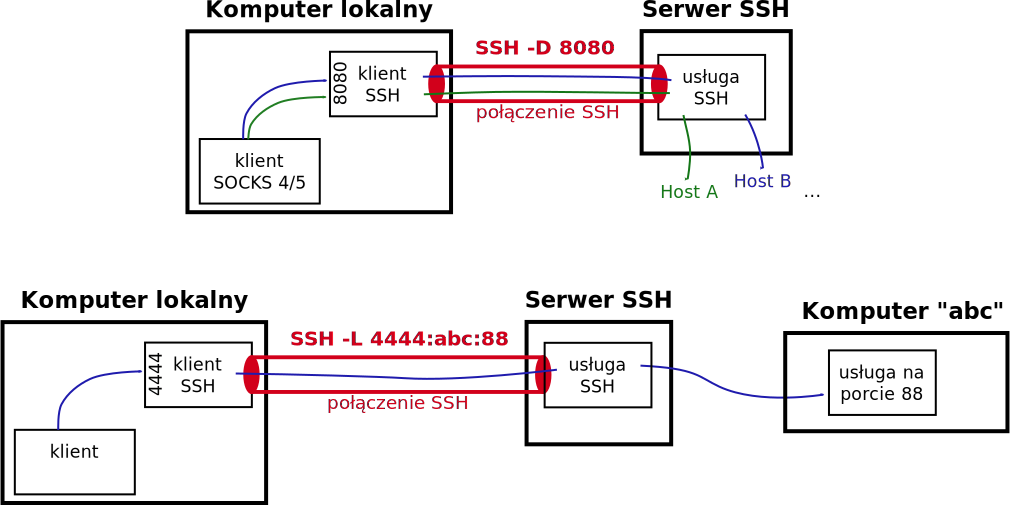
\includegraphics[width=0.7\textwidth]{img/linux/tunele_ssh}\end{center}
% END: ssh

% Copyright (c) 2017-2020 Matematyka dla Ciekawych Świata (http://ciekawi.icm.edu.pl/)
% Copyright (c) 2017-2020 Robert Ryszard Paciorek <rrp@opcode.eu.org>
% 
% MIT License
% 
% Permission is hereby granted, free of charge, to any person obtaining a copy
% of this software and associated documentation files (the "Software"), to deal
% in the Software without restriction, including without limitation the rights
% to use, copy, modify, merge, publish, distribute, sublicense, and/or sell
% copies of the Software, and to permit persons to whom the Software is
% furnished to do so, subject to the following conditions:
% 
% The above copyright notice and this permission notice shall be included in all
% copies or substantial portions of the Software.
% 
% THE SOFTWARE IS PROVIDED "AS IS", WITHOUT WARRANTY OF ANY KIND, EXPRESS OR
% IMPLIED, INCLUDING BUT NOT LIMITED TO THE WARRANTIES OF MERCHANTABILITY,
% FITNESS FOR A PARTICULAR PURPOSE AND NONINFRINGEMENT. IN NO EVENT SHALL THE
% AUTHORS OR COPYRIGHT HOLDERS BE LIABLE FOR ANY CLAIM, DAMAGES OR OTHER
% LIABILITY, WHETHER IN AN ACTION OF CONTRACT, TORT OR OTHERWISE, ARISING FROM,
% OUT OF OR IN CONNECTION WITH THE SOFTWARE OR THE USE OR OTHER DEALINGS IN THE
% SOFTWARE.

% BEGIN: zdalne kopiowanie
\subsection{zdalne kopiowanie}
Najprostszą metą kopiowania plików pomiędzy różnymi systemami jest wykorzystanie do tego ssh, typowo robi się to na jeden z 3 sposobów:
\begin{itemize}
	\item poleceniem
		\texttt{scp [opcje] źródło1 [źródło2 [...]] cel}
		, które
		kopiuje wskazany plik (lub pliki) do wskazanej lokalizacji, w przypadku kopiowania wielu plików cel powinien być katalogiem, do ważniejszych opcji należy zaliczyć:\\
		\texttt{-r} pozwala na (rekursywne) kopiowanie katalogów\\
		\texttt{-P port} określa port SSH\\
		W odróżnieniu od \texttt{cp} źródło lub cel w postaci \texttt{[user@]host:[ścieżka]} wskazują na zdalny system dostępny poprzez SSH.
	\item poleceniem
		\texttt{rsync [opcje] źródło cel}
		, które
		kopiuje (synchronizacjiuje) pliki i drzewa katalogów (zarówno lokalnie jak i zdalnie), do ważniejszych opcji należy zaliczyć:\\
			\texttt{-r} pozwala na (rekursywne) kopiowanie katalogów\\
			\texttt{-l} kopiuje linki symboliczne jako linki symboliczne (zamiast kopiowania zawartości pliku na który wskazują)\\
			\texttt{-t} zachowuje czas modyfikacji plików\\
			\texttt{-u} kopiuje tylko gdy plik źródłowy nowszy niż docelowy\\
			\texttt{-c} kopiuje tylko gdy plik źródłowy i docelowy mają inne sumy kontrolne\\
			\texttt{--delete} usuwa z docelowego drzewa katalogów elementy nie występujące w drzewie źródłowym\vspace{6pt}\\
			%
			\texttt{-e 'ssh'} pozwala na kopiowanie na/z zdalnych systemów za pośrednictwem ssh, źródło lub cel w postaci \texttt{[user@]host:[ścieżka]} wskazują na zdalny system
			\texttt{--partial --partial-dir=."-tmp-"} zachowuje skopiowane częściowo pliki w katalogu .-tmp- (pozwala na przerwanie i wznowienie transferu pliku)\\
			\texttt{--progress} pokazuje postęp kopiowania\\
			\texttt{--exclude="wzorzec"} pomija (w kopiowaniu i kasowaniu) pliki pasujące do wzorzec (wzorzec może zawierać znaki uogólniające powłoki)
			\texttt{-n} symuluje pracę (pokazuje co zostałoby skopiowane, ale nie kopiuje)
	\item złożonego polecenia opartego na przekierowaniu wyjścia jakiejś komendy do ssh, które uruchamia po zdalnej stronie proces odbierający te dane na swoim standardowym wejściu, np.:
		\begin{itemize}
			\item \Verb{tar -czf - ścieżka1 [ścieżka2 [...]] | ssh [user@]host 'cat > plik.tgz'}\\
				archiwizuje wskazane pliki/katalogi bezpośrednio na zdalny system z użyciem tar i kompresji gzip do pliku \texttt{plik.tgz}
			\item \Verb{tar -cf - ścieżka1 [ścieżka2 [...]] | ssh [user@]host 'tar -xf - -C cel'}\\
				kopiuje wskazane pliki/katalogi na zdalny system z użyciem tar do katalogu \texttt{cel}
		\end{itemize}
\end{itemize}
% END: zdalne kopiowanie 


% Copyright (c) 2017-2020 Matematyka dla Ciekawych Świata (http://ciekawi.icm.edu.pl/)
% Copyright (c) 2017-2020 Robert Ryszard Paciorek <rrp@opcode.eu.org>
% 
% MIT License
% 
% Permission is hereby granted, free of charge, to any person obtaining a copy
% of this software and associated documentation files (the "Software"), to deal
% in the Software without restriction, including without limitation the rights
% to use, copy, modify, merge, publish, distribute, sublicense, and/or sell
% copies of the Software, and to permit persons to whom the Software is
% furnished to do so, subject to the following conditions:
% 
% The above copyright notice and this permission notice shall be included in all
% copies or substantial portions of the Software.
% 
% THE SOFTWARE IS PROVIDED "AS IS", WITHOUT WARRANTY OF ANY KIND, EXPRESS OR
% IMPLIED, INCLUDING BUT NOT LIMITED TO THE WARRANTIES OF MERCHANTABILITY,
% FITNESS FOR A PARTICULAR PURPOSE AND NONINFRINGEMENT. IN NO EVENT SHALL THE
% AUTHORS OR COPYRIGHT HOLDERS BE LIABLE FOR ANY CLAIM, DAMAGES OR OTHER
% LIABILITY, WHETHER IN AN ACTION OF CONTRACT, TORT OR OTHERWISE, ARISING FROM,
% OUT OF OR IN CONNECTION WITH THE SOFTWARE OR THE USE OR OTHER DEALINGS IN THE
% SOFTWARE.

\section{Operacje na zawartości plików}

% BEGIN: grep
\subsection{grep i wyrażenia regularne}

Polecenie
\texttt{grep [opcje] wyrażenie [plik1 [plik2 [...]]]}
wyszukuje pasujące do wyrażenia regularnego wyrażenie linie w plikach, przydatne opcje:\\
	\texttt{-v} zamiast pasujących wypisz nie pasujące\\
	\texttt{-i} ignoruj wielkość liter\\
	\texttt{-a} przetwarzaj pliki binarne jak tekstowe\\
	\texttt{-E} korzystaj z ,,\emph{Extended Regular Expressions}'' (ERE) zamiast ,,\emph{Basic Regular Expressions}'' (BRE)\vspace{6pt}\\
	\texttt{-P} korzystaj z ,,\emph{Perl-compatible Regular Expressions}'' (PCRE) zamiast ,,\emph{Basic Regular Expressions}'' (BRE)\vspace{6pt}\\
	%
	\texttt{-r} rekursywnie przetwarzaj podane katalogi wyszukując w wszystkich znalezionych plikach\\
	\texttt{-R} jak -r, ale zawsze podąża za linkami symbolicznymi\\
	\texttt{--exclude="wyrażenie"} pomiń pliki pasujące do wyrażenie (może zawierać znaki uogólniające powłoki)\vspace{6pt}\\
	%
	\texttt{-l} wypisuje pliki z pasującymi liniami\\
	\texttt{-L} wypisuje pliki z bez pasujących linii

\vspace{13pt}\noindent Wyrażenia regularne\footnote{
	Podana składnia dotyczy ,,\emph{Extended Regular Expressions}'', przy BRE niektóre z znaków sterujących wymagają zabezpieczenia odwrotnym ukośnikiem.
} konstruuje się w oparciu o następujące znaki specjalne:
\vspace{-6pt}\begin{Verbatim}
.      - dowolny znak
[a-z]  - znak z zakresu
[^a-z] - znak z poza zakresu (aby mieć zakres z ^ należy dać go nie na początku)
^      - początek napisu/linii
$      - koniec napisu/linii

*      - dowolna ilość powtórzeń
?      - 0 lub jedno powtórzenie
+      - jedno lub więcej powtórzeń
{n,m}  - od n do m powtórzeń

()     - pod-wyrażenie (może być używane dla powtórzeń, a także referencji wstecznych)
\end{Verbatim}

\begin{teacherOnly}
Należy wspomnieć o historii, różnych formatach wyrażeń regularnych, kompatybilności wstecznej, czyli dlaczego
	\Verb#grep '^.\?$'# to to samo co \Verb#grep -E '^.?$'# i dlaczego w niektórych przypadkach stosujemy jedną a w innych inną notację.

Należy zwrócić uwagę na ,,pazerność'' dopasowań - na ogół dopasowawany najdłuższy możliwy fragment:\\
\Verb{echo '<a xx="oo" />bb<a yy="ii" />' | \grep -E --color '<a.*/>'} a:\\
\Verb{echo '<a xx="oo" />bb<a yy="ii" />' | \grep -E --color '<a[^>]*/>'} vs:\\
\Verb{echo '<a xx="oo" />bb<a yy="ii" />' | \grep -P --color '<a.*?/>'}

Wspomnieć także o opcji -x wymagającej dopasowania całej linii.
\end{teacherOnly}
% END: grep

\subsection{sed i inne narzędzia przetwarzania tekstów}
\begin{itemize}
	% BEGIN: sed
	\item \Verb{sed [opcje] [pliki]}
		edytuje plik zgodnie z podanymi poleceniami, przydatne opcje:\\
			\texttt{-e "polecenie"} - wykonuj na pliku polecenie (może wystąpić wielokrotnie celem podania wielu poleceń)\\
			\texttt{-f "plik"} - wczytaj polecenia z pliku plik\\
			\texttt{-E} - używaj rozszerzonych wyrażeń regularnych\\
			\texttt{-i} - modyfikuj podany plik zamiast wypisywać zmieniony na stdout\\
		przydatne polecenia:\\
			\texttt{s@regexp@napis@[g]} - wyszukaj dopasowania do wyrażenia regularnego regexp i zastąp je przez napis, podanie opcji g powoduje zastępowanie wszystkich wystąpień a nie tylko pierwszego, znak \texttt{@} pełni rolę separatora i może zostać zamiast niego użyty inny znak\\
			\texttt{y@zbiór1@zbiór2@} - zastąp znaki z zbiór1 znakami odpowiadającymi im pod względem kolejności znakami z zbiór2, znak \texttt{@} pełni rolę separatora i może zostać zamiast niego użyty inny znak\\
		możliwe jest też m.in. adresowanie linii na których ma być wykonywana operacja, np: \texttt{0,/regexp/ s@regexp@napis@} wykona polecenie s na liniach od początku pliku do linii pasującej do wyrażenia regularnego regexp, czyli zastąpi tylko pierwsze wystąpienie w pliku
	% END: sed
	
	\vspace{6pt}
	
	% BEGIN: tail head
	\item \Verb{tail [opcje] [plik]}
		wyświetla ostatnie linie pliku, przydatne opcje:\\
			\texttt{-n x} określa że ma zostać wyświetlone x ostatnich linii\\
			\texttt{-f} uruchamia dopisywania (gdy do pliku zostaną dopisane nowe linie tail je wyświetli)
	\item \Verb{head [opcje] [plik]}
		wyświetla początkowe linie pliku, przydatne opcje:\\
			\texttt{-n x} określa że ma zostać wyświetlone x pierwszych linii
	% END: tail head
	
	\vspace{6pt}
	
	% BEGIN: diff patch
	\item \Verb{diff ścieżka1 ścieżka2}
		porównuje pliki lub katalogi (w przypadku tych drugich porównuje ze sobą pliki o takich samych nazwach oraz zgłasza fakt występowania pliku tylko w jednym z katalogów), przydatne opcje:\\
			\texttt{-r} rekursywnie przetwarzaj podane katalogi\\
			\texttt{-u} wypisuje różnice w formacie "unified"\\
			\texttt{-c} wypisuje różnice w formacie "context"
	\item \Verb{patch}
	stosuje plik łaty (wynik diff'a) w celu zmodyfikowania plików, typowo:\\
		\texttt{patch -pn < plik.diff} co powoduje zastosowanie zmian opisanych w plik.diff na plikach w bieżącym katalogu,
		n określa ilość poziomów ścieżek podanych w pliku łaty które mają zostać zignorowane
	% END: diff patch
	% BEGIN: sort
	\item \Verb{sort [plik]}
		sortuje linie w wskazanym pliku, przydatne opcje:\\
			\texttt{-n} traktuj liczby jako wartości numeryczne a nie napisy\\
			\texttt{-i} ignoruj wielkość liter\\
			\texttt{-r} odwróć kolejność sortowania\\
			\texttt{-k n} sortuj wg kolumny n\\
			\texttt{-t sep} kolumny rozdzielane są przy pomocy separatora sep
	% END: sort
	
	\vspace{6pt}
	
	% BEGIN: cut
	\item \Verb{cut [opcje] [pliki]}
		wybiera z pliku zadany zestaw kolumn, przydatne opcje:\\
			\texttt{-f nnn} wypierz kolumny określone przez nnn (np. 1,3-4,6- oznacza kolumnę 1, kolumny od 3 do 4 i od 6, a -3 oznacza 3 pierwsze kolumny)\\
			\texttt{-d sep} kolumny rozdzielane są przy pomocy separatora sep (musi być pojedynczym jedno bajtowym znakiem, aby ominąć to ograniczenie należy skorzystać z awk)
	% END: cut
	% BEGIN: paste join comm uniq
	\item \Verb{paste}
		łączy (odpowiadające sobie pod względem numerów) linie z dwóch plików
	\item \Verb{join}
		łączy linie  z dwóch plików w oparciu o porównanie wskazanego pola
	\item \Verb{comm}
		porównuje dwa posortowane pliki pod względem unikalności linii (może wypisać wspólne lub występujące tylko w jednym z plików)
	\item \Verb{uniq}
		usuwa powtarzające się linie z posortowanego pliku, przydatne opcje:\\
			\texttt{-c} wypisz liczbę powtórzeń\\
			\texttt{-d} wypisz tylko linie z 2 lub więcej wystąpieniami\\
			\texttt{-u} wypisz tylko linie z 1 wystąpieniem
	% END: paste join comm uniq
\end{itemize}


\input{booklets-sections/linux/40-użytkownicy_uprawnienia_procesy.tex}
% Copyright (c) 2017-2020 Matematyka dla Ciekawych Świata (http://ciekawi.icm.edu.pl/)
% Copyright (c) 2017-2020 Robert Ryszard Paciorek <rrp@opcode.eu.org>
% 
% MIT License
% 
% Permission is hereby granted, free of charge, to any person obtaining a copy
% of this software and associated documentation files (the "Software"), to deal
% in the Software without restriction, including without limitation the rights
% to use, copy, modify, merge, publish, distribute, sublicense, and/or sell
% copies of the Software, and to permit persons to whom the Software is
% furnished to do so, subject to the following conditions:
% 
% The above copyright notice and this permission notice shall be included in all
% copies or substantial portions of the Software.
% 
% THE SOFTWARE IS PROVIDED "AS IS", WITHOUT WARRANTY OF ANY KIND, EXPRESS OR
% IMPLIED, INCLUDING BUT NOT LIMITED TO THE WARRANTIES OF MERCHANTABILITY,
% FITNESS FOR A PARTICULAR PURPOSE AND NONINFRINGEMENT. IN NO EVENT SHALL THE
% AUTHORS OR COPYRIGHT HOLDERS BE LIABLE FOR ANY CLAIM, DAMAGES OR OTHER
% LIABILITY, WHETHER IN AN ACTION OF CONTRACT, TORT OR OTHERWISE, ARISING FROM,
% OUT OF OR IN CONNECTION WITH THE SOFTWARE OR THE USE OR OTHER DEALINGS IN THE
% SOFTWARE.

\section{Inne polecenia}

Oprócz opisanych wcześniej najpopularniejszych / najistotniejszych poleceń istnieje wiele innych standardowych lub mniej standardowych (wymagających doinstalowania na wielu systemach) narzędzi linii poleceń. Poniżej wymienionych zostało kilka bardziej użytecznych przykładów.

Ponadto dowolny program w środowisku linuxowym (unixowym) może być uruchomiony z linii poleceń poprzez podanie jego nazwy (jeżeli jest w ścieżce wyszukiwania \Verb{$PARTH}) lub pełnej ścieżki do niego.
W bardzo wielu przypadkach takie uruchamianie pozwala przekazać do niego argument w postaci pliku do otwarcia lub inne opcje, czy nawet użycie programu normalnie pracującego z graficznym interfejsem użytkownika (takiego jak blender, inkscape, ...) w trybie nie interaktywnym (np. do automatycznej konwersji, itp.).

\begin{itemize}
	\item \Verb{date}
		data i czas, program ten potrafi także przeliczać datę i czas - np. \Verb$date -d @847103830 '+%Y-%m-%d %H:%M:%S'$, \Verb$date -d '1996-11-04 11:37:10' '+%s'$, \Verb$date -d '1996-11-04 11:37:10 +3week -2days'$
	\item \Verb{cal}
		kalendarz
	
	\item \Verb{wget} / \Verb{curl}
		pobieranie stron internetowych i plików
	
	\item \Verb{file}
		rozpoznaje typ pliku (w oparciu o zawartość)
	
	\item \Verb{convert}
		konwersje plików graficznych
	
	\vspace{6pt}
	
	\item \Verb{iconv}
		konwersje kodowań plików tekstowych
	\item \Verb{konwert}
		konwersje kodowań plików tekstowych – zarówno pomiędzy różnymi kodowaniami danego zbioru znaków, jak też pomiędzy kodowaniami nie pokrywającymi się czy też kodowaniami znaków 8 bitowych na mniejszej ilości bitów, na przykład://
			\Verb{konwert utf8-ascii} "inteligentnie" usunie znaki nie ascii z pliku kodowanego w utf-8 (np. znaczki z polskimi ogonkami zamieni na odpowiednie znaki ASCII bez tych ogonków);//
			\Verb{konwert qp-8bit} pozwoli zamienić kodowanie quoted printable na normalne 8 bitowe (rtf-8bit zrobi to z kodowaniem rtf'u)
		
	\item \Verb{mewencode} / \Verb{mewdecode}
		program (stanowiący część pakieu narzędzi dodatkowych dla kilenta pocztowego Mew) do obsługi kodowań mime (w tym Quoted-Printable, base64), m.in. zmienia kodowanie base64 na 8 bitowe
	\item \Verb{qprint}
		program do kodowania i dekodowania "Quoted-Printable"
	\item \Verb{base64}
		program do kodowania i dekodowania base64
	\item \Verb{strings}
		wypisuje sekwencje znaków drukowanych (określanie zawartości plików nietekstowych)
		
	\vspace{6pt}
	
	\item \Verb{command -v  komenda}
		zwraca wykonywaną ścieżkę / polecenie przy wykonywaniu \Verb{komenda}
\end{itemize}

% Copyright (c) 2017-2020 Matematyka dla Ciekawych Świata (http://ciekawi.icm.edu.pl/)
% Copyright (c) 2017-2020 Robert Ryszard Paciorek <rrp@opcode.eu.org>
% 
% MIT License
% 
% Permission is hereby granted, free of charge, to any person obtaining a copy
% of this software and associated documentation files (the "Software"), to deal
% in the Software without restriction, including without limitation the rights
% to use, copy, modify, merge, publish, distribute, sublicense, and/or sell
% copies of the Software, and to permit persons to whom the Software is
% furnished to do so, subject to the following conditions:
% 
% The above copyright notice and this permission notice shall be included in all
% copies or substantial portions of the Software.
% 
% THE SOFTWARE IS PROVIDED "AS IS", WITHOUT WARRANTY OF ANY KIND, EXPRESS OR
% IMPLIED, INCLUDING BUT NOT LIMITED TO THE WARRANTIES OF MERCHANTABILITY,
% FITNESS FOR A PARTICULAR PURPOSE AND NONINFRINGEMENT. IN NO EVENT SHALL THE
% AUTHORS OR COPYRIGHT HOLDERS BE LIABLE FOR ANY CLAIM, DAMAGES OR OTHER
% LIABILITY, WHETHER IN AN ACTION OF CONTRACT, TORT OR OTHERWISE, ARISING FROM,
% OUT OF OR IN CONNECTION WITH THE SOFTWARE OR THE USE OR OTHER DEALINGS IN THE
% SOFTWARE.

% BEGIN: System operacyjny - intro
\section{System operacyjny}
\begin{teacherOnly}
\begin{easylist}[itemize]
	& \textbf{proces startu}
		&& "co komputer zaczyna robić po włączeniu?"
		&& zasysanie instrukcji przez procesor
		&& załadowanie i uruchomienie bootloadera
		&& załadowanie i uruchomienie jądra
		&& opcja init
	& funkcje systemu operacyjnego
		&& procesy
			&&& co to jest proces
			&&& wątki (wątek vs proces)
			&&& \textbf{szeregowanie zadań}
			&&& drzewo procesów (rodzice)
			&&& ew. algorytmy szeregowania
			&&& fork()
			&&& sygnały
				&&&& kill
				&&&& czy proces może nie umrzeć? ... pokazać: wynik ps, wskazać pid bash'a, zrobić kill bash
				&&&& wiele różnych sygnałów ... Ctr+C ... Ctrl+Z ... info o zakończeniu potomka ...
		&& obsługa plików
			&&& wszystko jest plikiem
			&&& select(), czyli czekanie na dane ...
		&& \textbf{obsługa dostępu do pamięci}
			&&& pokazać rysując na tablicy stronnicowanie
			&&& pamięć współdzielona
				&&&& problem  if a==1: a=0
				&&&& semafory
		&& obsługa dostępu do urządzeń
			&&& interfejsy sieciowe, itd
		&& standardowe usługi
			&&& cron
			&&& mail
\end{easylist}
\end{teacherOnly}

System operacyjny jest programem uruchamianym po starcie komputera (co prawda nie jako pierwszym, ale zastępującym / usuwającym z pamięci uruchomione wcześniej, więc najstarszym z działających).
% END: System operacyjny - intro

% BEGIN: Proces uruchamiania komputera
\subsection{Proces startu}

Po otrzymaniu sygnału resetu (także przy uruchamianiu systemu - "Power-on Reset") procesor po inicjalizacji rejestrów zaczyna wykonywanie kodu znajdującego się pod jakimś ustalonym adresem (typowo w wbudowanej lub zewnętrznej pamięci typu ROM lub Flash). W zależności od danej architektury / procesrora może to być m.in.: bezpośrednio kod programu użytkownika, wbudowany bootloader danego procesora umożliwiający dalsze ładowanie np. z karty SD, zewnętrzny niskopoziomowy bootloader (np. u-boot).

W przypadku architektur zgodnych z x86 jest to BIOS, który po zakończeniu procesu inicjalizacji sprzętu i testów rozruchowych ładuje do pamięci kod znajdujący się w pierwszym sektorze dysku twardego (sektorze rozruchowym rozpoczynającym się od adresu zerowego) i uruchamia go (przekazuje do niego kontrolę). Znajduje się tam kod (lub tylko początek kodu) programu rozruchowego, którego zadaniem jest załadowanie systemu operacyjnego. W przypadku współczesnych systemów linuxowych jest to zazwyczaj GRUB.

Start systemu rozpoczyna się od załadowania do pamięci obrazu jądra wraz z parametrami oraz (opcjonalnie) initrd i przekazania kontroli do jądra przez program rozruchowy (np. GRUB). W przypadku jądra linuxowego i korzystania z initrd obraz ten przekształcany jest na RAM-dysk w trybie zapisu-odczytu i montowany jako rootfs z którego uruchamiany jest \Verb#/sbin/init# (którego podstawowym zadaniem jest zamontowanie właściwego rootfs). Po jego zakończeniu (lub od razu gdy nie używamy initrd) uruchamiany jest program wskazany w opcji \Verb#init=# jądra (domyślnie typowo \Verb#/sbin/init#) z rootfs wskazanego w opcji \Verb#root=# jądra. W opcji \Verb#init=# można wskazać dowolny program lub skrypt (uruchomiony zostanie z prawami root'a).
% END: Proces uruchamiania komputera

% BEGIN: Co robi system operacyjny
\subsection{Rola systemu operacyjnego}

System operacyjny jest oprogramowaniem odpowiedzialnym za zarządzanie zasobami systemu komputerowego (sprzętem, ale nie tylko) oraz uruchomionymi na nim aplikacjami. Do najistotniejszych zadań systemu operacyjnego zalicza się podział czasu procesora i szeregowanie zadań oraz zarządzanie pamięcią - w szczególności obsługa pamięci wirtualnej, najczęściej z wykorzystaniem mechanizmu stronicowania.

Oprócz tego system zajmuje się także zarządzaniem plikami, wejściem/wyjściem (najczęściej jest ono realizowane w oparciu o przerwania (IRQ), ale znane są także modele programowego we/wy polegającego na aktywnym czekaniu), obsługą urządzeń (wejście/wyjście, sterowniki, dostęp), obsługą sieci (stos protokołów sieciowych), itd.

Współczesne systemy korzystają z co najmniej dwóch poziomów pracy - uprzywilejowanego poziomu "nadzorcy" w którym działa jądro systemu operacyjnego oraz trybu użytkownika. Operacje I/O muszą odbywać się w trybie uprzywilejowanym. Również pamięć posiada obszar chroniony, w którym umieszczany jest m.in. tablica wektorów przerwań (inaczej zmiana adresu w tym wektorze mogłaby doprowadzić do przejęcia systemu w trybie uprzywilejowanym).
% END: Co robi system operacyjny

% BEGIN: Zarządzanie procesami
\subsubsection{Zarządzanie procesami}

Jednym z głównych zadań systemu operacyjnego jest zarządzanie procesami na nim uruchomionymi - obejmuje to zarówno czynności związane z ich tworzeniem oraz kończeniem, jak też szeregowanie zadań. To system operacyjny przejmuje okresowo procesor (z użyciem przerwania zegarowego), aby podjąć decyzję (w oparciu o jakiś algorytm szeregowania zadań) który/które z porcesów gotowych do działania (czyli takich, które aktualnie nie oczekują na "coś") ma dostać przydział czasu porcesora.
% END: Zarządzanie procesami

% BEGIN: Zarządzanie pamięcią
\subsubsection{Zarządzanie pamięcią}

Drugą podstawową funkcją systemu operacyjnego, wspomnianą na początku, jest zarządzanie pamięcią. Zarządzanie pamięcią polega na odpowiednim mapowaniu adresów logicznych (używanych przez procesy) na adresy fizyczne (używane przez procesor), korzysta ono z wsparcia sprzętowego ze strony procesora.

Jest to najczęściej realizowane w oparciu o wspomniany mechanizm stronicowania. Polega to na podziale pamięci dostępnej pamięci fizycznej na jednakowe bloki zwane ramkami oraz podziale pamięci logicznej na jednakowe bloki (o tej całej wielkości co ramki) zwane stronami. Strony które są wykorzystywane przez program są mapowane na dowolne ramki pamięci fizycznej (w przypadku gdy dana strona nie zamapowana - w zależności od okoliczności błąd braku strony lub błąd ochrony strony).

Rozwiązuje to problem fragmentacji zewnętrznej, polegającej na braku spójnego obszaru pamięci o żądanej długości pomimo iż łączna ilość wolnej pamięci jest dostateczna, jednak nie rozwiązuje problemu fragmentacji wewnętrznej, polegającej na przydzielaniu zbyt dużych fragmentów pamięci dla procesu (a wręcz można powiedzieć że go pogłębia).

Mechanizm ten wymaga trzymania tablicy wolnych ramek, tablicy stron dla każdego procesu (zawierającej przypisania mapowań stron danego procesu na ramki) oraz wykonywania tłumaczenia adresów logicznych (strona + przesunięcie na stronie). Także sama tablica stron procesu procesu może być stronicowania (mamy tablicę która informuje nas że przypisania stron w danym zakresie adresów są przechowywane w jakiejś ramce).

Strony i ramki mogą być współdzielone pomiędzy procesami (np. przy rozgałęzianiu procesu strony są kopiowane dopiero gdy zajdzie taka potrzeba). W przypadku braku miejsca w pamięci fizycznej wybrane strony nieaktywnego aktualnie procesu mogą być umieszczane na dysku (swap).
% END: Zarządzanie pamięcią

\subsubsection{Literatura dodatkowa {\Symbola 🤔}}

Było to bardzo krótkie i elementarne wprowadzenie w bardzo obszerny temat jakim są \textit{systemy operacyjne}. Wszystkich zainteresowanym niskopoziomowym działaniem systemu operacyjnego zachęcamy do zapoznania się z \href{https://pl.wikibooks.org/wiki/Pisanie_OS}{kursem pisania OS}\footnote{\url{https://pl.wikibooks.org/wiki/Pisanie_OS}} – niekoniecznie od razu pisania własnego systemu operacyjnego, ale przynajmniej zobaczeniem jak to się robi.


\section[Wykład wideo]{Wykład wideo\footnote{
	Filmy posiadają napisy wgrane do kontenera multimedialnego jako osobny strumień – napisy mogą być włączone lub wyłączone w odtwarzaczu.
	W wielu filmach dużo dzieje się "na dole ekranu", dlatego polecamy odtwarzać filmy z napisami umieszczonymi poniżej filmu, np. przy pomocy polecenia:
		\Verb$vlc --video-filter='croppadd{paddbottom=120}' --sub-margin=-10  PLIK.mkv$
}}

\input{booklets-sections/linux/wykład-video-1.tex}
\input{booklets-sections/linux/wykład-video-2.tex}
\input{booklets-sections/linux/wykład-video-3.tex}

\section{Literatura dodatkowa \zaawansowane{10}}
% Copyright (c) 2018-2020 Matematyka dla Ciekawych Świata (http://ciekawi.icm.edu.pl/)
% Copyright (c) 2018-2020 Robert Ryszard Paciorek <rrp@opcode.eu.org>
% 
% MIT License
% 
% Permission is hereby granted, free of charge, to any person obtaining a copy
% of this software and associated documentation files (the "Software"), to deal
% in the Software without restriction, including without limitation the rights
% to use, copy, modify, merge, publish, distribute, sublicense, and/or sell
% copies of the Software, and to permit persons to whom the Software is
% furnished to do so, subject to the following conditions:
% 
% The above copyright notice and this permission notice shall be included in all
% copies or substantial portions of the Software.
% 
% THE SOFTWARE IS PROVIDED "AS IS", WITHOUT WARRANTY OF ANY KIND, EXPRESS OR
% IMPLIED, INCLUDING BUT NOT LIMITED TO THE WARRANTIES OF MERCHANTABILITY,
% FITNESS FOR A PARTICULAR PURPOSE AND NONINFRINGEMENT. IN NO EVENT SHALL THE
% AUTHORS OR COPYRIGHT HOLDERS BE LIABLE FOR ANY CLAIM, DAMAGES OR OTHER
% LIABILITY, WHETHER IN AN ACTION OF CONTRACT, TORT OR OTHERWISE, ARISING FROM,
% OUT OF OR IN CONNECTION WITH THE SOFTWARE OR THE USE OR OTHER DEALINGS IN THE
% SOFTWARE.

\begin{itemize}
\item \textit{SSH jako VPN} (\url{http://blog.opcode.eu.org/2020/06/09/ssh_jako_vpn.html}) – opis konfiguracji tuneli SSH
\item \textit{Linux - podręcznik administratora sieci} (\url{http://www.interklasa.pl/portal/index/subjectpages/informatyka/linuxadm.pdf})
\item \textit{Introduction to TCP/IP} (\url{https://www.coursera.org/learn/tcpip/home/welcome}) – kurs na coursera.org
\end{itemize}


Więcej informacji o podstawach działania w systematach ,,unixowych'' oraz pełniejsza lista poleceń zamieszczona została pod adresem \url{http://vip.opcode.eu.org/#Systemy_unix-owate}.

\ZadaniaRozwiazaniaAuto[norepeat=true]

\copyrightFooter{
	© Matematyka dla Ciekawych Świata, 2017-2021.\\
	© Robert Ryszard Paciorek <rrp@opcode.eu.org>, 2003-2021.\\
	Kopiowanie, modyfikowanie i redystrybucja dozwolone pod warunkiem zachowania informacji o autorach.
}
\end{document}
